\documentclass[11pt, addpoints, answers]{exam}

\usepackage[utf8]{inputenc}
\usepackage[T1]{fontenc}
\usepackage[margin  = 1in]{geometry}
\usepackage{amsmath, amscd, amssymb, amsthm, verbatim}
\usepackage{mathabx}
\usepackage{setspace}
\usepackage{float}
\usepackage{color}
\usepackage{graphicx}
\usepackage[colorlinks=true]{hyperref}
\usepackage{tikz}

\usetikzlibrary{shapes,arrows}
%%%<
\usepackage{verbatim}
%%%>
\usetikzlibrary{automata,arrows,positioning,calc}

\usetikzlibrary{trees}

\shadedsolutions
\definecolor{SolutionColor}{RGB}{214,240,234}

\newcommand{\bbC}{{\mathbb C}}
\newcommand{\R}{\mathbb{R}}            % real numbers
\newcommand{\bbR}{{\mathbb R}}
\newcommand{\Z}{\mathbb{Z}}            % integers
\newcommand{\bbZ}{{\mathbb Z}}
\newcommand{\bx}{\mathbf x}            % boldface x
\newcommand{\by}{\mathbf y}            % boldface y
\newcommand{\bz}{\mathbf z}            % boldface z
\newcommand{\bn}{\mathbf n}            % boldface n
\newcommand{\br}{\mathbf r}            % boldface r
\newcommand{\bc}{\mathbf c}            % boldface c
\newcommand{\be}{\mathbf e}            % boldface e
\newcommand{\bE}{\mathbb E}            % blackboard E
\newcommand{\bP}{\mathbb P}            % blackboard P

\newcommand{\ve}{\varepsilon}          % varepsilon
\newcommand{\avg}[1]{\left< #1 \right>} % for average
%\renewcommand{\vec}[1]{\mathbf{#1}} % bold vectors
\newcommand{\grad}{\nabla }
\newcommand{\lb}{\langle }
\newcommand{\rb}{\rangle }

\def\Bin{\operatorname{Bin}}
\def\Var{\operatorname{Var}}
\def\Geom{\operatorname{Geom}}
\def\Pois{\operatorname{Pois}}
\def\Exp{\operatorname{Exp}}
\newcommand{\Ber}{\operatorname{Ber}}
\def\Unif{\operatorname{Unif}}
\def\No{\operatorname{N}}
\newcommand{\E}{\mathbb E}            % blackboard E
\def\th{\theta }            % theta shortcut
\def\V{\operatorname{Var}}
\def\Var{\operatorname{Var}}
\def\Cov{\operatorname{Cov}}
\def\Corr{\operatorname{Corr}}
\newcommand{\epsi}{\varepsilon}            % epsilon shortcut

\providecommand{\norm}[1]{\left\lVert#1\right\rVert} %norm
\providecommand{\abs}[1]{\left \lvert#1\right \rvert} %absolute value

\DeclareMathOperator{\lcm}{lcm}
\newcommand{\ds}{\displaystyle}	% displaystyle shortcut

\def\semester{2018-2019}
\def\course{Modèles Aléatoires Discrets}
\def\title{\MakeUppercase{Deuxième session}}
\def\name{Pierre-O Goffard}
%\def\name{Professor Wildman}

\setlength\parindent{0pt}

\cellwidth{.35in} %sets the minimum width of the blank cells to length
\gradetablestretch{2.5}

%\bracketedpoints
%\pointsinmargin
%\pointsinrightmargin

\begin{document}


\runningheader{\course  \vspace*{.25in}}{}{\title \vspace*{.25in}}
%\runningheadrule
\runningfooter{}{Page \thepage\ of \numpages}{}

% \firstpageheader{Name:\enspace\hbox to 2.5in{\hrulefill}\\  \vspace*{2em} Section: (circle one) TR: 3-3:50 \textbar\, TR: 5-5:50 \textbar\,  TR: 6-6:50(Xu) \textbar\,  TR: 6-6:50 }{}{Perm \#: \enspace\hbox to 1.5in{\hrulefill}\\ \vspace*{2em} Score:\enspace\hbox to .6in{\hrulefill} $/$\numpoints}
\extraheadheight{.25in}

\hrulefill

\vspace*{1em}

% Heading
{\center \textsc{\Large\title}\\
	\vspace*{1em}
	\course -- \semester\\
	Pierre-O Goffard\\
}
\vspace*{1em}

\hrulefill

\vspace*{2em}

\noindent {\bf\em Instructions:} On éteint et on range son téléphone.
\begin{itemize}
	\item La calculatrice et les appareils éléctroniques ne sont pas autorisés.
	\item Vous devez justifier vos réponses de manière claire et concise.
	\item Vous devez écrire de la manière la plus lisible possible. Souligner ou encadrer votre réponse finale.

\end{itemize}

\begin{center}
	\gradetable[h]
\end{center}

\smallskip

\begin{questions}
\question Soit $(X_n)_{n\geq0}$ une chaîne de Markov d'espace d'état $\{1,2,3,4\}$ de matrice de transition:
\[Q=\begin{pmatrix}
1/2 & 1/2 & 0 &0 \\
1-p & 0 & p&0 \\
0&1/2 &0& 1/2\\
0&0&1&0
\end{pmatrix},\text{ avec } 0\leq p\leq 1.
\]
	\begin{parts}
		\part[1]  Dessiner le graph des transitions de $(X_n)_{n\geq0}$
		\begin{solution}
			 \begin{center}
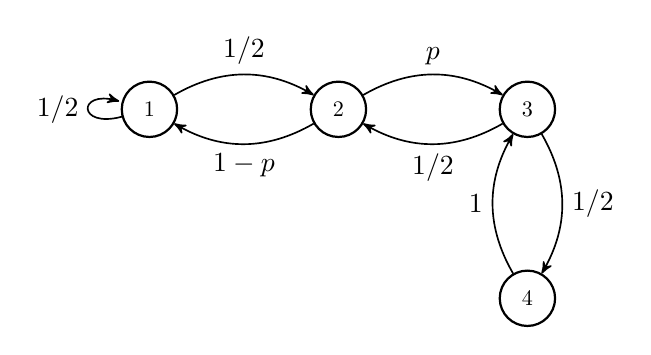
\begin{tikzpicture}[->, >=stealth', auto, semithick, node distance=3cm]
\tikzstyle{every state}=[fill=white,draw=black,thick,text=black,scale=0.8]
\node[state]    (1)                     {$1$};
\node[state]    (2)[right of=1]   {$2$};
\node[state]    (3)[right of=2]   {$3$};
\node[state]    (4)[below of=3]   {$4$};
\path

(1) edge[loop left]     node{$1/2$}         (1)
    edge[bend left]     node{$1/2$}         (2)

(2) edge[bend left]      node{$1-p$}      (1)
    edge[bend left]     node{$p$}         (3)
(3) edge[bend left]      node{$1/2$}      (2)
    edge[bend left]     node{$1/2$}      (4)
(4) edge[bend left]      node{$1$}      (3);

\end{tikzpicture}
\end{center}

		\end{solution}
		\part[3] Suivant les valeurs de $p$, donner les classes de communications et indiquer si elles sont ouvertes ou fermées.
		\begin{solution}
		\begin{itemize}
      \item Si $p = 0$, alors 2 classes de communications $F_1 = \{1,2\}$ fermée et $O_1 = \{3,4\}$ ouverte. 
      \item Si $p = 1$, alors 2 classes de communications $F_1 = \{2, 3, 4\}$ fermée et $O_1 = \{1\}$ ouverte
      \item Si $0<p< 1$, alors 1 classe de communications $F_1 = \{1,2, 3, 4\}$ fermée.
    \end{itemize}
		\end{solution}
		\part[3] Discuter l'existence et l'unicité de la loi stationnaire dans chacun des cas.
		\begin{solution}
		L'espace d'état est fini, il existe donc au moins une loi invariante dans chacun des cas. La loi stationnaire est unique dans le cas $0<p<1$ car la chaine est irréductible. Dans les deux autres cas, la présence d'une seule classe fermée implique que la loi stationnaire est unique aussi.
		\end{solution}

	\end{parts}
\question Au pays d'Oz, le temps ne peut prendre que $3$ formes : Beau temps
($B$), Pluvieux ($P$), ou Neigeux ($N$). Les règles d'évolution du
temps sont immuables et ne souffrent aucune exception.
\begin{itemize}
\item S'il fait beau, il ne fera pas beau le lendemain, et il y a
autant de chances qu'il pleuve ou qu'il neige le lendemain.
\item S'il pleut ou il neige, il y a une chance sur deux qu'il
fasse le même temps le lendemain, et une chance sur quatre qu'il
fasse beau le lendemain.
\end{itemize}
\begin{parts}
\part[2] Modélisez cette situation par une chaîne de Markov, et
justifiez ce choix. Donnez son graphe et sa matrice de transition.
\begin{solution}
La chaine de Markov donne la météo chaque jour, la météo d'un jour sur l'autre ne dépend que de la météo le jour précédent. Le graphe de transition est donné par
\begin{center}
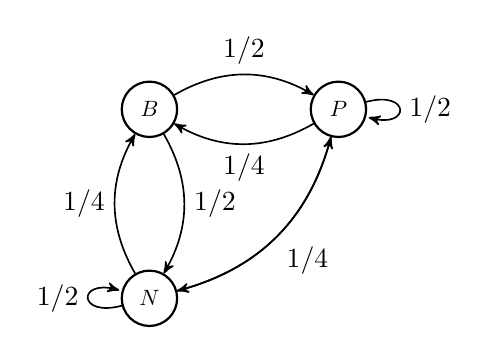
\begin{tikzpicture}[->, >=stealth', auto, semithick, node distance=3cm]
\tikzstyle{every state}=[fill=white,draw=black,thick,text=black,scale=0.8]
\node[state]    (1)               {$B$};
\node[state]    (2)[right of=1]   {$P$};
\node[state]    (3)[below of=1]   {$N$};
\path

(1) edge[bend left]     node{$1/2$}         (2)
    edge[bend left]     node{$1/2$}         (3)

(2) edge[loop right]     node{$1/2$}       (2)
    edge[bend left]     node{$1/4$}       (1)
    edge[bend left]     node{$1/4$}       (3)
(3) edge[loop left]     node{$1/2$}       (3)
    edge[bend left]     node{$1/4$}       (1)
    edge[bend right]     node{$$}       (2);
\end{tikzpicture}
\end{center}
et la matrice de transition est donnée par 
\[Q=\begin{pmatrix}
0 & 1/2 & 1/2  \\
1/4 & 1/2 & 1/4 \\
1/4&1/4 &1/2
\end{pmatrix}.
\]
\end{solution}
\part[2] Cette chaîne est-elle irréductible? Quelle est la nature des
états (récurrent ou transitoire)? leur période?
\begin{solution}
Une seule classe d'équivalence, la chaine est donc irréductible. Comme le nombre d'état est fini, les états sont récurrents. Finalement tout les états ont même période, celle ci est égale à $1$ puisque par exemple la transition $(P)\rightarrow(P)$ est possible.
\end{solution}
\part[2] Donnez, s'il en existe, la ou les mesures stationnaires de
cette chaîne.
\begin{solution}
La chaine est irréductible sur un espace d'état fini, on a donc existence et unicité de la loi stationnaire. Celle ci est obtenu en resolvant le système $\pi Q = \pi$, on a $\pi = \left(\frac{1}{5}\text{ }\frac{2}{5}\text{ }\frac{2}{5}\right)$
\end{solution}
\part[1] Quelle est la probabilité qu'il fasse beau après-demain
sachant qu'il fait beau aujourd'hui? 
\begin{solution}
On a $\mathbb{P}(X_{n+2} = B|X_{n} = B) = 1/4$. 
\end{solution}
\part[1] Après un certain temps (une fois que la chaine a atteint la stationarité), Quelle est la probabilité qu'il neige deux jours de suite en trois jours?
\begin{solution}
On peut initialiser l'état courant de la chaine suivant la loi stationaire $X_n\sim\pi$, on s'intéresse à l'évenement $E$ d'observer $2$ jours de neige sur une période de $3$ jours, on a 
$$
\mathbb{P}(E) = \sum_{i \in\{B,N,P\}}\mathbb{P}(E|X_n = i)\pi_i
$$  
On a 
$$
\mathbb{P}(E|X_n = N) = \mathbb{P}(X_{n+1} = N|X_n = N) = 1/2,
$$ 
$$
\mathbb{P}(E|X_n = B) = \mathbb{P}(X_{n+2} = N,X_{n+1} = N|X_n = B) = 1/4,
$$
$$
\mathbb{P}(E|X_n = P) = \mathbb{P}(X_{n+2} = N,X_{n+1} = N|X_n = P) = 1/8,
$$  
On en déduit que $\mathbb{P}(E) = 3/10$
\end{solution}
\part[2] En moyenne, combien de jours faut-il pour que le beau temps
revienne?\\

\underline{Indication:} On recherche $\mathbb{E}(\tau_B|X_0 =  B)$, avec $\tau_B=\inf\{n\geq1\text{ ; }X_n = B\}$. 
\begin{solution}
On note $\mathbb{E}_i(\tau_B) = \mathbb{E}(\tau_B|X_0 = i)$ et $\mathbb{P}(X_1 = j|X_0 = i)=\mathbb{P}(i,j)\text{, }i,j\in\{N,B,P\}$. On montre que
$$
\mathbb{E}_i(\tau_B) = \frac{3}{2}+\sum_{j\in\{N,B,P\}}\mathbb{P}(i,j)\mathbb{E}_j(\tau_B),\text{ }i\in\{N,B,P\},
$$
puis résoudre le système d'équation ou simplement écrire $\mathbb{E}(\tau_B|X_0 =  B) = 1 / \pi_B = 5$ par application du résultat du cours.
\end{solution}
\end{parts}


\question Soit la marche aléatoire sur $\mathbb{Z}$ définie par
$$
X_n = X_{n-1} + \xi_n,
$$ 
où $\xi_1,\xi_2\ldots$ forment une suite de variables aléatoires \textbf{i.i.d.} avec 
$$
\mathbb{P}(\xi_i = 1) = p\text{, et } \mathbb{P}(\xi_i = -1) = 1-p,\text{ pour tout }i\geq1\text{ et }0<p<1.
$$
On notera $q = 1-p$.
\begin{parts}
\part[1] Montrer que 
$$
\mathbb{E}(X_{n+1}|X_n) = X_n + 2p - 1.
$$
\begin{solution}
$$
\mathbb{E}(X_{n+1}|X_n) = \mathbb{E}(X_{n}+\xi_{n+1}|X_n) = X_n+\mathbb{E}(\xi_{n+1}) = X_n+ 2p -1
$$
\end{solution}
\part[1] Calculer $\mathbb{P}(X_2 = -2, X_5 = -1|X_0 = 0)$ en fonction de $p$ et $q$.
\begin{solution}
\begin{eqnarray*}
\mathbb{P}(X_2 = -2, X_5 = -1|X_0 = 0) &=& \mathbb{P}( X_5 = -3|X_2 = -2,X_0 = 0)\mathbb{P}(X_2 = -2|X_0 = 0) \\
 &=&\mathbb{P}( X_5 = -3|X_2 = -2)\mathbb{P}(X_2 = -2|X_0 = 0) \\
&=&\binom{3}{2}p^2q\binom{2}{0}q^2\\
&=&\binom{3}{2}p^2q^3\\
\end{eqnarray*}
\end{solution}
\part[1] Soit $T_5 = \inf\{n\geq0\text{ ; }X_n = 5\}$, calculer $\mathbb{P}(T_5 > 5|X_0 = 0)$ en fonction de $p$.
\begin{solution}
Conditionnellement à $X_0 = 0$, l'évènement $T_5<5$ est impossible. L'évènement $T_5=5$ correspond à $5$ saut vers le haut consécutif et correspond exactement à $X_5 = 5$. On a donc 
\begin{eqnarray*}
\mathbb{P}(T_5 > 5|X_0 = 0)&=&1-\mathbb{P}(T_5 \leq 5|X_0 = 0)\\
&=&1-\mathbb{P}(T_5 = 5|X_0 = 0)\\
&=&1-\mathbb{P}(X_5 = 5|X_0 = 0)\\
&=&1-p^5
\end{eqnarray*}  
\end{solution}
\end{parts}

\end{questions}
%-------------------------------TABLE-------------------------------
\newpage
\hrule
\vspace*{.15in}
\begin{center}
  \large\MakeUppercase{Formulaire}
\end{center}
\vspace*{.15in}
\hrule
\vspace*{.25in}

\renewcommand\arraystretch{3.5}
\begin{table}[H]
\begin{center}
\footnotesize
\begin{tabular}{|c|c|c|c|c|c|}

\hline
Nom & abbrev. & Loi & $\E(X)$ & $\Var(X)$ & FGM\\
\hline\hline
Binomial & $\Bin(n,p)$ & $\binom{n}{k}p^k(1-p)^{n-k}$ & $np$ & $np(1-p)$ & $[(1-p)+pe^t]^n$\\
\hline
Poisson & $\Pois(\lambda)$ & $e^{-\lambda}\dfrac{\lambda^k}{k!}$ & $\lambda$ & $\lambda$ &$ \exp(\lambda(e^t-1))$\\
\hline
Geometric & $\Geom(p)$ & $(1-p)^{k-1}p$ & $\dfrac{1}{p}$ & $\dfrac{1-p}{p^2}$ & $\frac{pe^t}{1-(1-p)e^t}$ pour  $t<-\ln(1-p)$\\
\hline
Uniform & $\Unif(a,b)$ & $\begin{cases} \dfrac{1}{b-a} & a\leq t\leq b\\ 0 & \text{sinon}\end{cases}
$ & $\dfrac{a+b}{2}$ & $\dfrac{(b-a)^2}{12}$ & $\frac{e^{tb}-e^{ta}}{t(b-a)}$\\
\hline
Exponential & $\Exp(\lambda)$ & $\begin{cases} \lambda e^{-\lambda t} & t\geq 0 \\ 0 & t<0\end{cases}$ & $\dfrac{1}{\lambda}$ & $\dfrac{1}{\lambda^2}$ & $\frac{\lambda}{\lambda -t}$ pour $t<\lambda$\\
\hline
Normal & $\No(\mu,\sigma^2)$ & $\left(\dfrac{1}{\sqrt{2\pi\sigma^2}}\right)\operatorname{exp}{\left(\dfrac{-(t-\mu)^2}{2\sigma^2}\right)}$ & $\mu$ & $\sigma^2$ & $e^{\mu t}e^{\sigma^2t^2/2}$\\
\hline
\end{tabular}
\end{center}
\end{table}%

\textbf{Théorème Central Limite.}\\
Soient $X_1,\ldots,X_n$ une suite de $n$ variables aléatoires \textbf{i.i.d.} telles que $\mu =\mathbb{E}(X_1)$ et $\sigma^{2} =\mathbb{V}(X_1)<\infty$. Alors, on a
$$
\frac{\sqrt{n}}{\sigma}(\bar{X}_n-\mu)\overset{\text{Loi}}{\rightarrow}\No(0,1),\text{ lorsque }n\rightarrow\infty,
$$
où $\bar{X}_n=\frac{1}{n}\sum_{k=1}^{n}X_k$ désigne la moyenne empirique.

\end{document}